\section{Introduction}\label{sec_introduction}

%Many modern machine learning methods
%Hard parameter sharing (HPS) for multi-task learning is widely used in empirical research and goes back to the seminal work of \cite{C97}.
%Recent work has revived interests in this approach because it improves performance and reduces the cost of collecting labeled data \cite{R17}.
%It is generally applied by sharing the feature layers between all tasks while keeping an output layer for every task.
%Often, hard parameter sharing offers two critical advantages if successfully applied.
%First, it reduces model parameters since all tasks use the same feature space.
%Second, it reduces the amount of labeled data needed from each task by augmenting the entire training dataset.

%Hard parameter sharing works as an inductive transfer mechanism and a regularizer that reduces overfitting, both of which have great intuitive appeal \cite{R17}.
%For example, by restricting the shared space's size, HPS encourages information sharing among multiple tasks \cite{KD12}.
%Another source of inductive bias comes from the tasks and depends on datasets' properties such as sample sizes and task covariances \cite{WZR20}.
%However, how these dataset properties impact HPS has not been well established.
%It becomes increasingly important to understand HPS' formal generalization properties.
%Part of the challenge may be that HPS' generalization performance depends intricately on the sample size ratios and covariate shifts between tasks, and is not amenable to standard concentration results.
%Previous results based on Rademacher complexity or VC dimensions have considered cases where all tasks' sample sizes are equal to logarithmic factors of the feature dimension \cite{B00,MPR16}, and when all tasks' sample sizes increase simultaneously \cite{AZ05,M06}.
%For, the generalization error scales down as the sample sizes of all tasks increase, when applied to the multi-task setting \cite{B00,AZ05,M06,MPR16,WZR20}.

%This paper presents new techniques to study hard parameter sharing and establishes a number of new results.
%We consider regression analysis, which is arguably one of the most fundamental problems in statistics and machine learning.
%We are interested in the \textit{high-dimensional} setting, where each dataset's sample size and feature dimension grow linearly instead of logarithmically.
%This setting captures the fact that a single task's sample size is usually insufficient for accurate learning in many applications.
%For example, if a dataset's sample size is only a constant factor of dimension in linear regression, the variance is also constant (cf. Fact \ref{fact_tr}).
%The high-dimensional setting is challenging but is crucial for understanding how datasets' sample sizes impact generalization performance.


\subsection{Setup and motivating examples}

We first define the data model.
Suppose we have two datasets (or tasks).
We refer the first dataset as the source and the second task as the target.
Let $i = 1$ or $2$.
Let $n_i$ be dataset $i$'s sample size.
Let $x_1^{(i)}, x_2^{\ss (i)}, \dots, x_{n_i}^{(i)}$ be the $n_i$ datapoints' $p$-dimensional covariates.
Let $y_1^{(i)}, y_2^{(i)}, \dots, y_{n_i}^{(i)}$ be these datapoints' labels.
We assume a linear model specified by an unknown model vector $\beta^{(i)} \in \real^p$ as follows:
\begin{align}
    y_j^{(i)} = \inner{x_j^{(i)}}{\beta^{(i)}} + \varepsilon_j^{(i)}, \text{ for any } j = 1,\dots,n_i, \label{eq_linear}
\end{align}
where $\varepsilon^{(i)}_j$ denotes an additive noise (independent of the covariates).
%Let $(x_1^{(2)}, y_1^{(2)}), \dots, (x_{n_2}^{(2)}, y_{n_2}^{(2)})$ be $n_2$ labeled examples, where $x_i^{(2)}$ denotes the covariates and $y_i^{(2)}$ denotes the label, for any $i = 1,\dots, n_2$.
%Similar to the first dataset, we assume that
%for an unknown vector $\beta^{(2)}\in\real^p$ and an additive noise $\varepsilon^{(2)}_i$.
Our goal is to learn an estimator to predict the target task given both datasets.

We consider a high-dimensional setting on each dataset where the sample size $n_i$ increases with $p$ to infinity proportionally by a constant factor, which has recently received lots of interests (see e.g., \citet{hastie2019surprises} and Section \ref{sec_related} for more references).
Let $\Sigma^{(i)} \in \real^{p\times p}$ be a deterministic positive semidefinite matrix.
The covariates are assumed to have population covariance equal to $\Sigma^{(i)}$:
\begin{align}
    x_j^{(i)} = \big(\Sigma^{(i)}\big)^{1/2} z_{j}^{(i)}, \text{ for any } j = 1,\dots,n_i, \label{eq_rvm}
\end{align}
where $z_j^{(i)}$ consists of independent and identical entries sampled from a distribution that has zero mean, unit variance, and satisfies certain bounded moment condition. 
We focus on the so called \textit{underparametrized} setting for task two where $n_2 > \rho p$ for a constant $\rho > 1$ whereas for task one $n_1$ can be smaller than $p$.
See Section \ref{sec_data} for the precise assumptions underlying the above data model.

We learn a two-layer linear neural network with parameters $A \in \real^{p\times r}$, $B_1 \in \real^{r}$, and $B_2 \in \real^r$ by minimizing the following optimization objective:
\begin{align}\label{eq_hps}
    f(A, B_1, B_2) = \bignorm{X^{(1)} A B_1 - Y^{(1)}}_2^2 + \bignorm{X^{(2)} A B_2 - Y^{(2)}}_2^2.
\end{align}
The above two-layer neural network uses a shared feature space $A$ for both tasks while using a separate prediction head for each task.\footnote{A popular variant of objective function \eqref{eq_hps} adds a weight parameter to each summand. We focus on the unweighted objective for simplicity and all of our results apply to the weighted objective.}
Such models are also known as \textit{hard parameter sharing} in the machine learning literature \cite{C97,R17}.
Suppose that $(\hat{A}, \hat{B}_1, \hat{B}_2)$ is a global minimizer of $f(\cdot)$.
We define the hard parameter sharing (HPS) estimator for the target task as $\hat{\beta}_2^{\MTL} \define \hat{B} \hat{A}_2$.
In order to evaluate the estimator, we will study the excess risk at a new (unseen) test datapoint from task two, denoted as $L(\hat{\beta}_2^{\MTL})$ (see Section \ref{sec_risk} for its precise definition).

As a motivating example of the above setup, we show an intriguing simulation where combining both datasets jointly results in different transfer effect on $L(\hat{\beta}_2^{\MTL})$, depending on the distance between $\beta^{(1)}$ and $\beta^{(2)}$.
Figure \ref{fig_motivation} shows the result for a setting where every entry of $X_1, X_2$ is generated from an isotropic Gaussian, and $\beta_1,\beta_2$ are generated such that $\norm{\beta^{(1)} - \beta^{(2)}}^2 \approx 2\mu^2$.
We observe that for $\mu = 0.25$, $L(\hat{\beta}_2^{\MTL})$ is always smaller than the excess risk of OLS.
For the other $\mu$ values, $L(\hat{\beta}_2^{\MTL})$ is smaller than the excess risk of OLS for a restricted range of $n_1$.
Such a scenario, where combining both datasets jointly improves over learning the target task individually, and is also called a \textit{positive information transfer} \cite{PY09}.
Our main contribution is to precisely analyze a number of interesting phenomena including the above that are prevalent in transfer learning, depending on geometries of the covariance matrices and model distances. 


\begin{figure*}
    \centering
    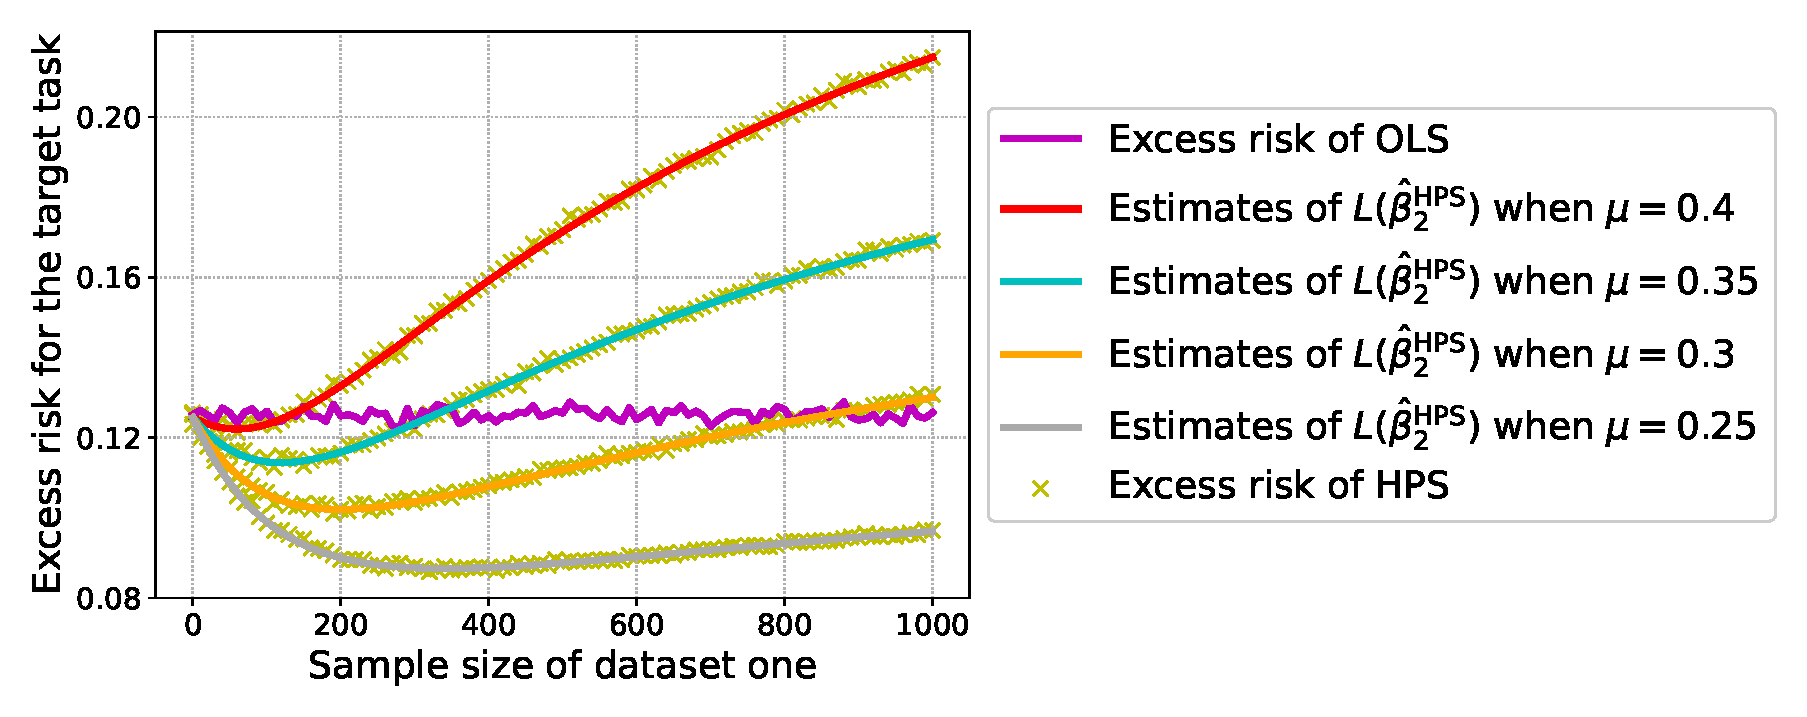
\includegraphics[width=0.7\textwidth]{figures/motivation.eps}
    \caption{We illustrate that our setup can reproduce the phenomenon of \textit{positive} (or \textit{negative}) \textit{information transfer}, which is prevalent in the context of transfer learning.
    We vary the sample size of dataset one and the distance parameter $\mu$ such that $\norm{\beta^{(1)} - \beta^{(2)}}^2 = 2\mu^2$. The region below the excess risk of the ordinary least squares (OLS) estimator corresponds to the range of $n_1$ in which $L(\hat{\beta}_2^{\MTL})$ is smaller than the excess risk of the OLS estimator. See also Figure \ref{fig_ab_data} for a similar phenomenon observed in text classification tasks.}
    \label{fig_motivation}
\end{figure*}

\subsection{Summary of results}
%\todo{mention connection to pooling \cite{hanneke2020no}}

\paragraph{Precise asymptotics given heterogeneous sources.}
Having defined the data model for each task, next, we describe typical scenarios in transfer learning under our setup.
We define two settings as follows:
\begin{itemize}
    \item \textbf{Covariate shift:}
    independent $X^{(1)}$ and $X^{(2)}$ with the same population covariance matrices but different models.
    Our second result (Theorem \ref{thm_main_RMT}) applies to two tasks with arbitrarily different sample size ratios and covariate shifts.
    While we can no longer characterize $f(A, B)$'s global minimum because of non-convexity, we can still provide a sharp bias-variance tradeoff of any local minimizer's prediction loss for both tasks.
    Despite being a simple setting, we observe several non-trivial phenomena by varying sample size ratios and covariate shifts between the two tasks.
    \item \textbf{Model shift:} independent $X^{(1)}$ and $X^{(2)}$ with the same population covariance matrices (i.e. $\Sigma^{(1)}=\Sigma^{(2)}$) but different models (i.e. $\beta^{(1)} \neq \beta^{(2)}$).
    \item \textbf{Covariate and model shift.}
\end{itemize}

Theoretical insights
\begin{itemize}
    \item \textit{Whether or not covariate shift helps depends on sample sizes:} In addition to sample sizes, variance also scales with two datasets' covariate shifts. For a large sample size ratio, HPS's  variance is smallest when there is no covariate shift. Counterintuitively, for a small sample size ratio, having covariate shifts reduces variance through a complementary spectrum. We achieve this result through a novel characterization on the inverse of the sum of two sample covariance matrices with arbitrary covariate shifts. See our discussion of proof techniques below for details.
    \item \textit{Identical covariance provides approximately optimal transfer under imbalanced sizes:}
    \item \textit{Determining information transfer under model shift}: Increasing one task's sample size does not always reduce another task's loss. In a simplified setting, we find that the task loss either decreases first before increasing afterward or decreases monotonically depending on how fast the bias grows. These two trends result from different bias-variance tradeoffs. This result is surprising because previous generalization bounds in multi-task learning typically scale down as all tasks' sample sizes increase, thus do not apply for different sample size ratios.
\end{itemize}

\paragraph{Empirical results.}
Finally, we discuss the practical implications of our work.
Our sample size ratio study implies a concrete progressive training procedure that gradually adds more data until performance drops.
For example, in the setting of Figure \ref{fig_intro_sample_size_b}, this procedure will stop right at the minimum of the local basin.
We conduct further studies of this procedure on six text classification datasets and observe that it reduces the computational cost by $65\%$ compared to a standard round-robin training procedure while keeping the average accuracy of all tasks simultaneously.


\paragraph{Extension to multiple sources.}
Our first result (Theorem \ref{thm_many_tasks}) applies to multi-label prediction settings where all datasets have the same features (and sample size), and we want to make several predictions for every input (cf. examples in \cite{hsu2009multi}).
We analyze the global minimizer of $f(A, B)$, and provide a sharp bias-variance decomposition of its (out-of-sample) prediction loss for any task.
This setting is tractable even though in general, $f(A, B)$ is non-convex in $A$ and $B$ (e.g. matrix completion is a special case for suitably designed $X^{(i)}, Y^{(i)}$).
%We show that the prediction loss of HPS admits a clean bias-variance decomposition.
Our result implies that when all tasks have the same features but different labels, for any task, HPS helps reduce the task's variance compared to single-task learning but increases bias.


%See Figure \ref{fig_intro_sample_size_b} for an illustration of the former.
Consequently, using our precise loss estimates, we observe several qualitative properties of HPS for varying dataset properties.
%\begin{itemize}
%	\item \textit{Sample efficiency (Example \ref{ex_same_cov})}:
%	One advantage of combining multiple datasets is that the requirement for labeled data reduces compared to single-task learning, a phenomenon that \cite{ZSSGM18} has observed empirically.
%	Our results further imply that HPS's sample efficiency depends on model-specific variances across tasks vs. the noise variance and is generally high when the latter is large.



%\end{itemize}

%\medskip
%\noindent\textbf{Proof techniques.}
%There are two main ideas in our analysis. The proof of our first result uses a geometric intuition that hard parameter sharing finds a ``rank-$r$'' approximation of the datasets.
%We carefully keep track of the concentration error between the global minimizer of $f(A, B)$ and its population version (cf. equation \eqref{eq_A_star}).
%The proof of our second result is significantly more involved because of different sample sizes and covariate shifts. We show that the inverse of the sum of two sample covariance matrices with arbitrary covariate shifts converges to a deterministic diagonal matrix asymptotically (cf. Theorem \ref{thm_main_RMT}).
%We use recently developed techniques from random matrix theory to show a sharp convergence rate.
% to obtain a sharp estimate on the..., which is commonly referred to as the \emph{local law}.
%\HZ{add several sentences on the technical insight}
%One limitation of our analysis is that in Example \ref{ex_sample_ratio}, there is an error term that can result in vacuous bounds for very small $n_1$ (cf. equation \eqref{cor_MTL_error}).
%We believe our result has provided significant initial insights, and it is an interesting question to tighten our result.
%See Section \ref{sec_conclude} for more discussions of the technical challenge.



\subsection{Related work}\label{sec_related}


\paragraph{Sample covariance matrices with distribution shift.}
These previous works mainly consider cases with only one high-dimensional sample covariance matrix involved. %need to check 
In the single task case, if the data is Gaussian, then the precise variance limit can be derived directly from properties of Wishart distribution. In the high-dimensional setting, the eigenvalues of Wishart matrices satisfy the famous Marchenko–Pastur (MP) law \cite{MP}, whose Stieltjes transform characterizes the variance limit. Furthermore, it is well-known that the MP law holds universally regardless of the detailed data distribution \cite{bai2010spectral}. \cite{isotropic} obtained a sharp converge rate of the empirical spectral distribution (ESD) to the MP law for sample covariance matrices with isotropic covariance. \cite{Anisotropic,DY} later extended this result to sample covariance matrices with arbitrary population covariances. These results are proved by establishing certain optimal convergence estimates of the Stieltjes transforms of sample covariance matrices, which are referred to as \emph{local laws} in the random matrix theory literature. We refer the reader to \cite{erdos2017dynamical} and the references therein for a detailed review of related concepts. We extend these techniques to the two-task setting and prove a local law for the sum of two sample covariance matrices with an arbitrary covariate shift, which is one technical contribution of this work. From the local law, we can derive the variance limit with a precise dependence on the singular values of the covariate shift matrix. 

%Our proof techniques use the so-called local law of random matrices, a recent development in the random matrix theory literature, called the \emph{local law} of 

%These techniques provide almost sharp convergence rates to the asymptotic limit compared to other methods such as free probability \cite{nica2006lectures}.
%We also extend the techniques in ?, which is one contribution of this work. 

%On the other hand, one may derive the asymptotic result in Theorem \ref{thm_main_RMT} with error $\oo(1)$ using the free addition of two independent random matrices in theory.

There is another method to derive the asymptotic variance limit using free addition in free probability theory \cite{nica2006lectures}. We do not take this procedure because this method is not completely justified in the general non-Gaussian setting with non-diagonal covariate shift matrix. 
%(in the sense that it is hard to establish rigorously the free independence between two sample covariance matrices). 
Furthermore, our techniques provide almost sharp convergence rates to the asymptotic limit, which is not given by free probability techniques. 

On the other hand, the bias limit is much harder to study, and its dependence on the sample ratio and the covariate shift is still an open problem in random matrix theory in the most general setting. However, when the data is Gaussian distributed and the two tasks have the same population covariance, we find a way to calculate the exact bias limit using free probability techniques. Leveraging on the recent results \cite{BES_free1,BES_free2}, we can obtain a sharp convergence rate to the bias limit. To the best of our knowledge, we are not aware of any previous result on the precise bias limit in the high-dimensional setting, even for two Wishart matrices with the same population covariance matrix. 

\paragraph{Random matrix theory and machine learning.} \todo{write a paragraph regarding applications of RMT to modern machine learning.}
\begin{itemize}
	\item \citet{hastie2019surprises}
	\item \citet{bartlett2020benign}
	\item \citet{liang2020just}
	\item \citet{montanari2019generalization}, \citet{liang2020precise}
\end{itemize}
\begin{remark}
    \todo{clarify overparametrize}
    As a clar,  following the work of \citet{hastie2019surprises} (see also \citet{bartlett2020benign} and the references therein)
\end{remark}


\paragraph{Transfer learning and related problems.}
There is a large body of classical and recent works on multi-task learning.
The early work of \cite{B00,BS03,M06} studied multi-task learning from a theoretical perspective, often using uniform convergence or Rademacher complexity based techniques.
An influential paper by \cite{BBCK10} provides uniform convergence bounds that combine multiple datasets in certain settings.
One limitation of uniform convergence based techniques is that the results often assume that all  tasks have the same sample size, see e.g. \cite{B00,MPR16}.
\citet{pontil2013excess}
Moreover, these techniques do not apply to the high-dimensional setting because the results usually require a sample size of at least $p \log p$.
The problem we study here is also related to high-dimensional prediction in transfer learning \cite{li2020transfer,bastani2020predicting}.
For example, \cite{li2020transfer} provide minimax-optimal rates to predict a target regression task given multiple sparse regression tasks.
One closely related work is \cite{WZR20}, which studied hard parameter sharing for two linear regression tasks.
However, their results only apply to sample size regimes at least logarithmic factors of dimension.
\todo{a list of relevant papers}
\begin{itemize}
	\item \citet{lei2021nearoptimal}
	\item \citet{kalan2020minimax}
	\item  \citet{cai2021transfer}
	\item \citet{lounici2011oracle}
\end{itemize}
\textit{Other related works.} Distributed learning \cite{dobriban2018high}.

%Linear models in multi-task learning have been studied in various settings, including online learning \cite{CCG10,DCSP18}, sparse regression \cite{LPTV09,LPVT11}, and representation learning \cite{BHKL19}.

%Our setting is closely related to domain adaptation \cite{DM06,BB07,BC08,DH09,MMR09,CWB11,ZS13,NB17,ZD19}.
%The important distinction is that we focus on predicting the target task using a hard parameter sharing model.
%For such models, their output dimension plays an important role of regularization \cite{KD12}.
%Below, we describe several lines of work that are most related to this work.

%Some of the earliest works on multi-task learning are Baxter , Ben-David and Schuller \cite{BS03}.
%Mauer \cite{M06} studies generalization bounds for linear separation settings of MTL.
%The benefit of learning multi-task representations has been studied for learning certain half-spaces \cite{MPR16} and sparse regression \cite{LPTV09,LPVT11}.
%Our work is closely related to Wu et al. \cite{WZR20}.
%While Wu et al. provide generalization bounds to show that adding more labeled helps learn the target task more accurately, their techniques cannot be used to explain when MTL outperforms STL.
%\todo{spell out the challenge more explicitly}

%Ando and Zhang \cite{AZ05} introduces an alternating minimization framework for learning multiple tasks.
%Argyriou et al. \cite{AEP08} present a convex algorithm which learns common sparse representations across a pool of related tasks.
%Evgeniou et al. \cite{EMP05} develop a framework for multi-task learning in the context of kernel methods.
%\cite{KD12} observed that controlling the capacity can outperform the implicit capacity control of adding regularization over $B$.
%The multi-task learning model that we have focused on uses the idea of hard parameter sharing \cite{C93,KD12,R17}.
%We believe that our theoretical framework can apply to other approaches to multi-task learning.


\subsection{Organizations}
The rest of this paper is organized as follows.
In Section \ref{sec_HPS}, we formally define the data model and describe the underlying assumptions.
We show a bias-variance decomposition of the HPS estimator, and connect the bias and variance equations to random matrix theory.
In Section \ref{sec_main}, we show precise estimates for the excess risk of the HPS estimator under covariate and model shifts.
In Section \ref{sec_exp}, we evaluate the performance of HPS estimators against several commonly used transfer learning estimators, and present two implications for migating covariate and model shift in neural networks.
In Section \ref{sec_same}, we extend our setup to transferring from multiple data sources under model shift.
Section \ref{sec_conclude} concludes the paper and discusses potential future directions.
Section \ref{app_proof_error_same_cov}, \ref{appendix RMT}, and \ref{app_iso_cov} present proofs of our results.